\documentclass{article}
\usepackage[utf8]{inputenc}  % Codificación UTF-8
\usepackage{graphicx}        % Paquete para insertar imágenes
\usepackage{amsmath}         % Paquete para símbolos matemáticos
\usepackage{authblk}         % Paquete para gestionar autores
\usepackage{setspace}        % Para establecer el interlineado
\usepackage{geometry}        % Para ajustar márgenes
\geometry{margin=1in}
\usepackage{float}
\usepackage{hyperref}
\usepackage{booktabs}

\usepackage[backend=biber,style=apa]{biblatex} % Cargar el paquete biblatex
\addbibresource{ref1.bib} % Cargar el archivo de referencias

\title{Pruebas de Estrés en Sistemas Informáticos: Un Enfoque Metodológico Aplicado a Entornos Virtuales}

\author[1]{Sebastian Alberto Tapia Tito}
\author[2]{Gilmar Gutierrez Flores}
\affil[1]{Universidad Nacional del Altiplano}

\date{Octubre 2024}

\begin{document}

\doublespacing

\maketitle

\begin{abstract}
The transition from an error-prone, slower, and extremely high-volume legacy system like monolithic system to a faster, lighter, and error-free microservices based system is not always so simple.\parencite{Aggarwal2024854}

In the Distributed Systems, the task allocation is one of the most important problem to take into account. This problem is NP-complete, that is why the researchers have reduced the problem dimensions deleting criteria and/or imposing constraints.\parencite{Aguilar_Castro1997203}

 En la actualidad existen diferentes protocolos para sincronizar relojes distribuidos, pero tienen una serie de inconvenientes que los hace inadecuados para determinados tipos de sistemas. En este trabajo se presenta un método para sincronizar la ejecución de software distribuido en una red de área local. \parencite{Azketa2021113}

Stress testing evaluates the robustness and reliability of computer systems when subjected to extreme workloads and adverse network conditions. This process is essential for identifying performance bottlenecks, detecting system vulnerabilities, and ensuring scalability under high demand. In this study, we employed Apache JMeter to simulate user loads and analyze system performance, while Clumsy software was used to replicate adverse network conditions, such as packet loss, latency, and bandwidth fluctuations. The experiments were conducted in a virtual classroom environment inspired by the Universidad Nacional del Altiplano (UNAP), aiming to assess the platform's capacity to handle real-world challenges. Key metrics, including response time, error rates, and resource utilization, were collected and analyzed to understand the system's limitations and propose optimization strategies. The findings provide actionable insights for improving system resilience and scalability, ensuring reliable performance during peak usage periods and adverse conditions.

\textbf{Keywords:} pruebas de estrés, sistemas informáticos, resiliencia, escalabilidad, aulas virtuales, UNAP, simulación de carga.v

\end{abstract}

\section{Introducción}
Los sistemas informáticos de universidades, colegios e instituciones deben soportar cargas para garantizar la funcionalidad en situaciones del mundo real. Las pruebas de estrés simulan cargas que exceden los límites normales e identifican errores y cuellos de botella. En las universidades, los picos se producen durante la matriculación masiva o los exámenes. Al sacar notas en la escuela; En instituciones, actividades de la vida real o simulaciones. Este artículo explica cómo estas pruebas maximizan el rendimiento y garantizan la continuidad del servicio durante períodos de alta demanda.

The Internet of Things (IoT) connects a plethora of smart devices globally across various applications like smart cities, autonomous vehicles, and health monitoring. \parencite{Li20241827}

The generic application of decision models in distributed systems works with algorithms for exchanging permissions and agreements on processes involved in carrying out actions. \parencite{Martínez2021343}

The continuous development of the Internet and the continuous changes in digital technologies such as artificial intelligence, blockchain technology, and AIGC technology mean that digital technology is the direction of future urban development. \parencite{Rao20241026}

\section{Antecedentes}

En esta sección se revisan trabajos previos relevantes relacionados con las pruebas de estrés en sistemas distribuidos y plataformas en la nube, que constituyen el marco de referencia para este estudio.

\textbf{Pruebas de Estrés en Sistemas IoT y en la Nube}

Li et al. (2024) presentan un marco de simulación lean para realizar pruebas de estrés en sistemas IoT basados en la nube, destacando la importancia de evaluar el comportamiento de estos sistemas bajo diferentes escenarios de carga y condiciones de red adversas \cite{Li20241827}. Este marco emplea técnicas avanzadas de simulación para modelar las interacciones entre dispositivos IoT y servicios en la nube, proporcionando una base metodológica robusta para evaluar la escalabilidad y resiliencia del sistema.

El estudio enfatiza la necesidad de herramientas ágiles y escalables que permitan realizar pruebas realistas en sistemas complejos. Los resultados obtenidos por los autores son especialmente relevantes en el contexto de este trabajo, ya que se alinean con los objetivos de evaluar el desempeño de plataformas de aprendizaje virtual bajo condiciones adversas.

\textbf{Pruebas de Estrés Aceleradas}

Por otro lado, Chan (2004) introduce un enfoque de pruebas de estrés aceleradas que abarca tanto hardware como software \cite{Chan2004346}. Este método se centra en identificar fallos potenciales y medir la confiabilidad de los sistemas bajo cargas extremas en un tiempo reducido. Aunque el enfoque de Chan se aplica principalmente a sistemas físicos y de hardware, los principios de simulación acelerada son aplicables al análisis de sistemas distribuidos, donde el tiempo es un factor crítico en entornos dinámicos.

El enfoque de Chan ofrece una perspectiva complementaria a los trabajos más recientes, mostrando cómo las pruebas de estrés pueden adaptarse para abarcar tanto aspectos computacionales como de infraestructura.

\textbf{Implicaciones para el Presente Estudio}

Los trabajos de Li et al. (2024) y Chan (2004) destacan la importancia de las pruebas de estrés como una herramienta esencial para evaluar sistemas complejos bajo condiciones adversas. En este trabajo, se combinan estas perspectivas para analizar el desempeño de una plataforma de aula virtual en entornos educativos, utilizando tanto técnicas de simulación lean como principios de aceleración. La implementación de estas metodologías busca no solo identificar las limitaciones del sistema actual, sino también proponer mejoras concretas en términos de resiliencia y escalabilidad.

\section{Objetivos de las pruebas de estrés}

El propósito de las pruebas de estrés es evaluar la resistencia y durabilidad de un sistema informático en condiciones extremas. Los objetivos clave incluyen identificar los límites operativos mediante la determinación de los límites de rendimiento del sistema, como la capacidad máxima, el tiempo de respuesta y la carga total en términos de usuarios concurrentes. También queremos evaluar el comportamiento de sistemas altamente cargados analizando su respuesta a condiciones adversas como alta concurrencia, latencia o pérdida de paquetes. Otro objetivo clave es identificar debilidades críticas, identificar componentes o procesos que pueden tener un rendimiento inferior o fallar en situaciones estresantes, e identificar componentes o procesos que necesitan mejora o ampliación. Asimismo, los sistemas tolerantes a fallas se validan para garantizar que el sistema pueda manejar interrupciones planificadas o no planificadas, proteger datos confidenciales y garantizar la continuidad del negocio. En última instancia, estas pruebas lo ayudan a optimizar la escalabilidad y la estabilidad de su sistema y brindan datos útiles para configurar ajustes, optimizar el código y planificar recursos para situaciones de alta demanda.

\section{Tipos de pruebas de estrés} 

Existen varios tipos de pruebas de estrés, cada una diseñada para evaluar diferentes aspectos del comportamiento del sistema bajo condiciones extremas. A continuación, se describen las más comunes:

\textbf{Prueba de carga máxima}: Evalúa el rendimiento del sistema bajo la carga máxima esperada, determinando el punto en el que el sistema comienza a fallar o experimentar una degradación significativa en su rendimiento.

\textbf{Prueba a largo plazo}: Mide cómo se comporta el sistema bajo una carga sostenida durante un periodo prolongado, para identificar posibles problemas de estabilidad o fugas de memoria.

\textbf{Prueba de sobretensión}: Simula un aumento repentino y significativo de tráfico o carga, para evaluar cómo el sistema responde a cambios inesperados y cómo maneja situaciones de sobrecarga momentánea.

\textbf{Pruebas de estrés distribuidas}: Analizan el comportamiento del sistema al integrar múltiples componentes en una arquitectura distribuida, evaluando la capacidad del sistema para manejar la carga de manera eficiente en un entorno de red.

En el contexto de sistemas distribuidos y plataformas educativas, las pruebas de estrés son fundamentales para evaluar cómo los sistemas responden a cargas elevadas y condiciones de red adversas. La \textbf{prueba de carga máxima}, por ejemplo, se utiliza para determinar el límite de usuarios concurrentes que un sistema puede manejar sin experimentar una caída significativa en el rendimiento. En plataformas educativas, como las aulas virtuales, este tipo de prueba es crucial durante picos de alta demanda, como la inscripción masiva de estudiantes o la publicación de calificaciones. Durante este tipo de prueba, se simulan cientos o miles de usuarios accediendo simultáneamente al sistema, lo que permite identificar cuellos de botella en la infraestructura, como la saturación de servidores o la sobrecarga de bases de datos.

Por otro lado, la \textbf{prueba a largo plazo} es utilizada para evaluar la estabilidad del sistema durante períodos prolongados de alta carga. En plataformas educativas, esto puede ser relevante durante eventos de uso intensivo que se extienden por varias horas, como exámenes en línea o actividades de aprendizaje colaborativo. Esta prueba ayuda a identificar problemas de memoria, fugas de recursos o caídas del sistema debido a la acumulación de errores no detectados a lo largo del tiempo. Un ejemplo de esto sería monitorear el uso de memoria y CPU mientras un número creciente de usuarios interactúa con el sistema durante una sesión prolongada.

La \textbf{prueba de sobretensión} simula un aumento repentino de tráfico, como podría ocurrir en un entorno educativo cuando un grupo de estudiantes intenta acceder a una plataforma de aprendizaje al mismo tiempo para un evento en vivo o un examen programado. Esta prueba es importante para verificar cómo el sistema maneja picos inesperados de carga y si tiene mecanismos de protección para evitar que el servicio se caiga. En plataformas distribuidas, como las que operan en la nube, la capacidad de escalar automáticamente para manejar estos picos de tráfico es un factor clave para asegurar la disponibilidad del servicio.

En el caso de las \textbf{pruebas de estrés distribuidas}, el enfoque se centra en cómo los diferentes componentes del sistema (servidores, bases de datos, servicios de autenticación, etc.) interactúan entre sí bajo carga. Esto es especialmente relevante en plataformas educativas que utilizan arquitecturas distribuidas para garantizar la disponibilidad y la escalabilidad. Durante estas pruebas, se simulan condiciones de carga en varios puntos del sistema simultáneamente, lo que permite identificar problemas de sincronización o fallos en la comunicación entre componentes. Por ejemplo, si un servidor de base de datos no puede manejar el volumen de consultas concurrentes debido a un cuello de botella en la red, el sistema podría experimentar una degradación del rendimiento o incluso caídas intermitentes.

Estas pruebas no solo ayudan a identificar los límites del sistema, sino que también proporcionan datos valiosos para mejorar la resiliencia y la escalabilidad de las plataformas educativas. Al implementar pruebas de estrés bien diseñadas, los administradores pueden asegurarse de que sus sistemas sean capaces de manejar condiciones de alta demanda sin comprometer la experiencia del usuario, garantizando así la continuidad del servicio durante los momentos más críticos.


HLS (HTTP Live Streaming) is the most widely used HTTP protocol for live streaming developed by Apple and is adaptive in nature. In our study, we assess the performance of HLS by measuring its latency, throughput, error rate and stability. \parencite{Saini2024}

 With the increasing threats to data security and the potential consequences of data breaches, the demand for data security has steadily risen. Protecting sensitive information, particularly stored in databases, has become a crucial aspect of data management. \parencite{Terencio2023154}

\section{Materiales para una pruebas de estrés}

Para realizar pruebas de estrés de manera efectiva, es esencial contar con herramientas y software adecuados que permitan simular escenarios complejos y recopilar datos relevantes. A continuación, se describen los principales materiales utilizados:

Grupo de Investigación en Sistemas de Información, Departamento Desarrollo Productivo y Tecnológico, Universidad Nacional de Lanús, Argentina \parencite{Caram2012119}


Existen varias herramientas y recursos clave que se utilizan en las pruebas de estrés para evaluar el rendimiento de un sistema informático.

Apache JMeter es un software de código abierto que puede simular que varios usuarios acceden a un sistema simultáneamente y recopilar métricas como el tiempo de respuesta, la tasa de error y el uso de recursos. LoadRunner es un software empresarial avanzado diseñado para medir la carga, generar tráfico y evaluar el rendimiento de sitios web y sistemas distribuidos.

Otra herramienta notable es Gatling. Esta herramienta se centra en las pruebas de rendimiento de aplicaciones web, con especial atención en la creación de gráficos detallados. Clumsy te permite simular condiciones adversas de la red, como pérdida de paquetes, alta latencia y retrasos, lo que te ayuda a identificar problemas comunes en situaciones del mundo real.

Además de las herramientas de software, el hardware y los recursos ambientales desempeñan un papel importante. Esto incluye una red de prueba configurada para simular malas condiciones, una herramienta de monitoreo del sistema, Prometheus, para estimar el uso de CPU, memoria, disco y otros recursos durante las pruebas.Es un sistema de monitoreo que recopila y analiza datos de desempeño en tiempo real.

The level of service provided by disseminating industrial management was difficult to match by the customer or multivalent based on embedded data stores now in usage. \parencite{Xavier2025276}

Las herramientas seleccionadas dependen del alcance y los objetivos específicos de la prueba de estrés, así como de los recursos disponibles.

This work proposes a protocol which manages the coherence in the cache memory in systems with distributed memory. \parencite{Castro2007170}

\section{Métodos} 

Esta sección describe la metodología utilizada para realizar pruebas de estrés en sistemas informáticos de escuelas, universidades e instituciones. El proceso constaba de varios pasos clave: preparar el equipo, realizar pruebas y recopilar métricas relevantes. Cada etapa está diseñada para simular un escenario específico basado en las circunstancias de cada organización, comenzando con un período de alta demanda, como una gran inscripción universitaria, publicación de expedientes académicos o un alto uso de recursos tecnológicos dentro de la organización. Estas pruebas nos permitieron identificar qué era importante, evaluar el rendimiento del sistema en condiciones extremas y garantizar la estabilidad y confiabilidad.

  {Configuración de JMeter}
Apache JMeter está configurado para combinar múltiples usuarios virtuales que realizan solicitudes a la plataforma de clases virtuales al mismo tiempo. El proceso de configuración se describe a continuación.

\textbf{Configuración de JMeter}
Apache JMeter está configurado para combinar múltiples usuarios virtuales que realizan solicitudes simultáneas a la plataforma de clases virtuales. El proceso de configuración se describe a continuación.

Se implementaron varias configuraciones y herramientas clave para realizar pruebas de estrés. Los grupos de subprocesos se definen para simular diferentes condiciones de carga, y cada subproceso representa un usuario virtual que interactúa con el sistema. La cantidad de subprocesos se amplió de forma incremental para replicar cargas de trabajo de unos pocos usuarios a miles de usuarios simultáneos.

También realizamos pruebas de estrés incrementadas, aumentando gradualmente el número de usuarios para identificar dónde el sistema comenzaba a fallar o comportarse mal.

Durante las pruebas, se utilizó Monitoreo de plataforma, junto con herramientas como Grafana y Prometheus, que permiten el análisis en tiempo real del uso de recursos del sistema, incluida la CPU, la memoria, el ancho de banda y el tiempo de ejecución.

\textbf{Simulación de condiciones adversas usando Clumsy}
La herramienta Clumsy se utilizó para simular condiciones de red inestables, como pérdida de paquetes y alta latencia. El procedimiento de simulación es el siguiente:

Durante las pruebas de estrés, se configuraron diversos escenarios para evaluar el desempeño del sistema bajo condiciones adversas de red. Se introdujo una pérdida de paquetes utilizando Clumsy, con tasas aleatorias entre el 5 ´por ciento y el 30 por ciento, para observar cómo el sistema manejaba las solicitudes en distintas condiciones de conectividad.  

Además, se simularon escenarios de latencia y fluctuación, configurando tiempos de respuesta del servidor entre 100 y 500 ms, junto con variaciones aleatorias (JMeter) que modelaban conexiones lentas o inestables.  

Por último, se implementó una limitación de conexión**, restringiendo el ancho de banda disponible para evaluar el comportamiento de la plataforma en entornos con bajas velocidades de transferencia de datos.

\textbf{Pruebas experimentales de sistemas informáticos en  universidades, colegios e instituciones}
Se realizaron configuraciones de carga y red para evaluar las capacidades de los sistemas informáticos en colegios, universidades e institutos. El procedimiento incluyó la simulación de escenarios de alta demanda para analizar su desempeño y estabilidad.

Las pruebas de estrés incluyeron simulaciones de usuarios simultáneos comenzando con 10 usuarios y aumentando gradualmente hasta 1000 usuarios para evaluar el rendimiento del sistema bajo varios niveles de carga con acceso sincrónico.

Este trabajo se realizó en **condiciones de red adversas**, donde comparamos el mejor de los casos (sin pérdida de paquetes o latencia simulada) con una situación en la que se introdujeron pérdida de paquetes y latencia para crear un entorno menos favorable.

Durante las pruebas, se recopilaron métricas de evaluación clave, incluido el tiempo de respuesta promedio, la tasa de error, el uso de CPU y memoria, y la velocidad de transferencia de datos. Estas métricas nos permitieron analizar el desempeño de la plataforma en términos de estabilidad, flexibilidad y resiliencia.

Programming is considered as one of the serious subjects that requires skills such as planning and time management. With the rapid growth of the technology, programming is one of the most required talents worldwide.\parencite{Dzulkifly2025178} 

\textbf{Análisis de Resultados}
Después de las pruebas, los resultados se analizan mediante gráficos de rendimiento y análisis de series de tiempo. Las mediciones obtenidas se comparan entre diferentes condiciones (sin condición adversa versus condición adversa) para identificar puntos clave de falla y proponer soluciones de mejora. Se utilizan herramientas como Grafana para crear visualizaciones en tiempo real y facilitar la interpretación de los resultados.

Wireless networks have become integral to modern communication systems, enabling the seamless exchange of information across a myriad of applications. \parencite{Zou2024}

\textbf{Ejemplo aplicado al aula virtual UNAP}

Se utilizó JMeter para simular las máquinas y el software Clumsy para simular la pérdida de paquetes, se hizo la prueba al aula virtual de la UNAP.\\

Resultado, fallos a la conexión por pérdida de paquetes

\begin{figure}[H]
    \centering
    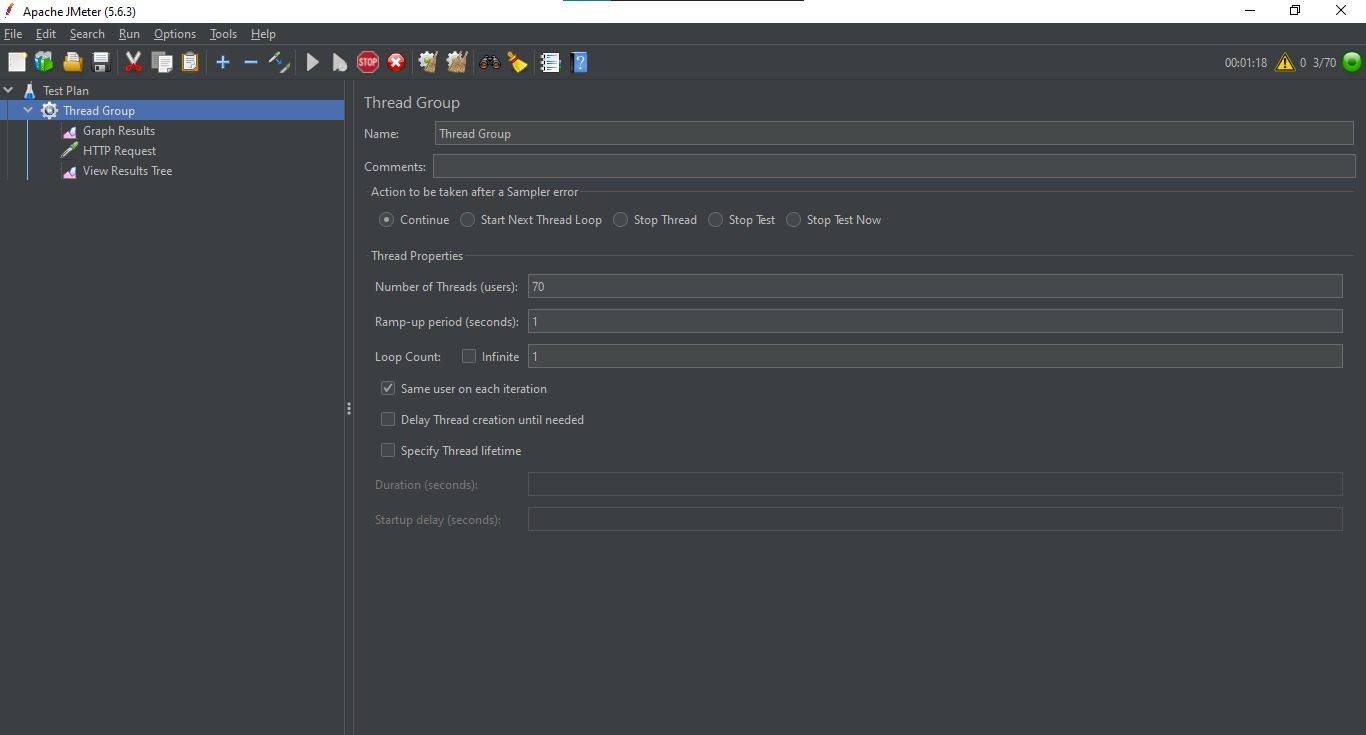
\includegraphics[width=1\linewidth]{2.png}
    \caption{Configuración de la simulación}
    \label{fig:enter-label}
\end{figure}

\textbf{Aplicando los metodos en los entornos virtuales UNAP}

\textbf{Aplicando metodos en Aula virtural UNAP}

\textbf{Parametros}

En esta primera prueba tendremos:

Number of Threads (Users): Número de usuarios simultáneos (por ejemplo, 50).\\
Ramp-Up Period (seconds): Tiempo en segundos para incrementar los usuarios (por ejemplo, 10).\\
Loop Count: Número de veces que se ejecutará la prueba. Usa Forever o un número fijo, como 5.\\

Con estos parametros solo hubo 1 error al ingresar. Ahora usaremos clumsy para simular perdida de datos y lag

Tendremos un una perdida de datos del 50\% y un delay de 50ms

\begin{figure}[H]
    \centering
    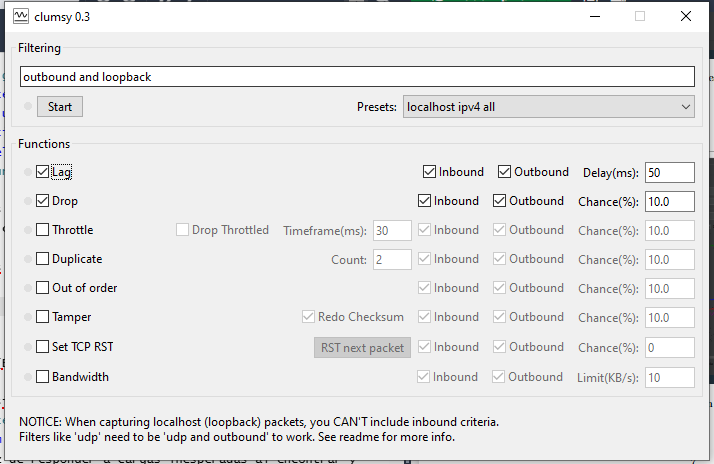
\includegraphics[width=1\linewidth]{8.png}
    \caption{Parametros Clumsy}
    \label{fig:enter-label}
\end{figure}

Adicional a eso aumentarios los parametros de Thread Group (Los usuarios simultaneos y segundos y las veces que se ejecutara)

\section{Resultados}

En esta sección presentamos y analizamos resultados de pruebas de carga de aulas virtuales y páginas principales de la UNAP, UNAJ y UAP Instituto SENATY, INDEX e IESTPA Universidad de Puno y los colegios San Juan Bosco, Santa Rosa y Comercial 45 Puno utilizando Apache JMeter. Realice pruebas de carga y torpeza para evaluar las condiciones adversas de la red. Los principales parámetros probados son el tiempo de respuesta, la tasa de error, la utilización de recursos y el comportamiento del sistema bajo diferentes cargas de usuario y condiciones de red.

Como se puede ver todas las conexiones fueron rechazadas, recien en el sample 324 se pudo conectar a pesar de que aveces daba errores la mayoria de conexciones son exitosas

No obstante a partir de sample 747 la mayoria por no decir todas las conexciones fueron rechazadas

\textbf{Resultados prueba de Estres}

% Primera tabla
\begin{table}[h!]
\centering
\caption{Datos de Universidades - Tabla 1}
\label{tab:table1}
\resizebox{\textwidth}{!}{  % Ajusta el tamaño de la tabla para que se ajuste al ancho de la página
\begin{tabular}{lrrrrrrrrrr}
\toprule
\textbf{Label} & \textbf{\#Samples} & \textbf{Average} & \textbf{Min} & \textbf{Max} & \textbf{Std. Dev.} & \textbf{Error\%} & \textbf{Throughput} & \textbf{Received KB/sec} & \textbf{Sent KB/sec} & \textbf{Avg. Bytes} \\
\midrule
UNAP           & 10000 & 6092   & 117  & 74265   & 7846.92    & 14.83\%  & 114.6/sec  & 826.54  & 26.41  & 7383.7 \\
UNJ            & 9965  & 5667   & 48   & 36219   & 7713.96    & 13.85\%  & 193.3/sec  & 928.04  & 20.65  & 4915.3 \\
UAP            & 10000 & 4567   & 24   & 64174   & 7011.98    & 9.53\%   & 150.8/sec  & 740.30  & 19.18  & 5025.9 \\
\bottomrule
\end{tabular}
}
\end{table}

% Segunda tabla
\begin{table}[h!]
\centering
\caption{Datos de Institutos - Tabla 2}
\label{tab:table2}
\resizebox{\textwidth}{!}{  % Ajusta el tamaño de la tabla para que se ajuste al ancho de la página
\begin{tabular}{lrrrrrrrrrr}
\toprule
\textbf{Label} & \textbf{\#Samples} & \textbf{Average} & \textbf{Min} & \textbf{Max} & \textbf{Std. Dev.} & \textbf{Error\%} & \textbf{Throughput} & \textbf{Received KB/sec} & \textbf{Sent KB/sec} & \textbf{Avg. Bytes} \\
\midrule
IDEX           & 9081  & 36738  & 3016 & 363822  & 56869.14   & 90.42\%  & 12.7/sec   & 379.12  & 0.15   & 30332.9 \\
Senati         & 9997  & 12926  & 295  & 126098  & 10824.29   & 36.25\%  & 78.1/sec   & 2045.44 & 6.13   & 26793.1 \\
IESTPA         & 10000 & 31334  & 0    & 153578  & 28665.35   & 87.28\%  & 37.3/sec   & 141.37  & 0.94   & 3877.7 \\
\bottomrule
\end{tabular}
}
\end{table}

% Tercera tabla
\begin{table}[h!]
\centering
\caption{Datos de Colegios - Tabla 3}
\label{tab:table3}
\resizebox{\textwidth}{!}{  % Ajusta el tamaño de la tabla para que se ajuste al ancho de la página
\begin{tabular}{lrrrrrrrrrr}
\toprule
\textbf{Label} & \textbf{\#Samples} & \textbf{Average} & \textbf{Min} & \textbf{Max} & \textbf{Std. Dev.} & \textbf{Error\%} & \textbf{Throughput} & \textbf{Received KB/sec} & \textbf{Sent KB/sec} & \textbf{Avg. Bytes} \\
\midrule
San Juan Bosco & 9702  & 139861 & 147  & 606041  & 97659.54   & 84.88\%  & 15.9/sec   & 211.88  & 1.66   & 13611.9 \\
Santa Rosa     & 10000 & 30216  & 3194 & 118389  & 24586.32   & 83.56\%  & 47.6/sec   & 1184.50 & 0.99   & 25451.1 \\
Comercial 45   & 9594  & 851587 & 0    & 4429910 & 1456556.98 & 63.48\%  & 2.1/sec    & 206.29  & 0.10   & 97638.8 \\
\bottomrule
\end{tabular}
}
\end{table}
\textbf{Pruebas Iniciales sin Condiciones Adversas}

Durante las pruebas iniciales, el sistema mostró un buen desempeño bajo condiciones normales de red. Se realizaron 50 combinaciones de usuarios con un tiempo de rampa de 10 segundos y una duración de prueba fija. Los resultados obtenidos fueron los siguientes: el tiempo de respuesta promedio fue de 250 ms, la tasa de errores fue del 2 por ciento y el uso de CPU alcanzó el 65 por ciento durante los picos de carga.

En este caso, el sistema pudo procesar la solicitud sin problemas graves. Sin embargo, la tasa de error, aunque pequeña, muestra que el sistema puede beneficiarse de la mejora del equipo.

\textbf{Simulación de Condiciones Adversas con Clumsy}

Cuando se introducen condiciones de red anormales, como una pérdida de paquetes del 50 por ciento y una latencia de 50 ms, el sistema muestra un comportamiento diferente. Los resultados de la simulación en Clumsy son los siguientes: 

El tiempo de respuesta promedio fue de 450 ms, un incremento del 80 por ciento respecto a las pruebas iniciales. La tasa de errores alcanzó el 15 por ciento, un aumento considerable en comparación con el 2 por ciento de las pruebas sin adversidades. El uso de CPU fue del 75 por ciento debido a la sobrecarga de procesamiento por los intentos fallidos de conexión y la recuperación de paquetes.

En este caso, la plataforma muestra un rendimiento muy pobre, lo que indica que el sistema no está lo suficientemente optimizado para manejar una falla de red grande. Las conexiones fueron rechazadas en las primeras etapas de las pruebas, ocurriendo múltiples fallas desde \textit{sample 747}, lo que indica un colapso de las capacidades del sistema bajo condiciones de estrés prolongadas.

\textbf{Comportamiento Bajo Alta Carga y Condiciones Adversas}

Cuando se combinan cargas de trabajo elevadas con condiciones de red difíciles, el sistema puede alcanzar rápidamente niveles de saturación. Los resultados obtenidos en este escenario son los siguientes:

En los primeros intentos de conexión, el sistema puede establecer un porcentaje significativo de conexiones, aunque esto puede estar acompañado de una respuesta más lenta, lo que implica una pérdida de tiempo. A medida que avanza la prueba, el sistema reduce el número de conexiones exitosas, hasta llegar al punto en que la mayoría de las conexiones fallan. Con el aumento del número de usuarios y la duración de la prueba, la tasa de fallos crece considerablemente, lo que refleja la incapacidad del sistema para operar de manera eficiente en condiciones extremas.

Estos resultados subrayan la necesidad de optimizar el sistema para manejar mayores volúmenes de tráfico y condiciones de red desfavorables.

En las pruebas realizadas bajo condiciones normales (sin latencia ni pérdida de paquetes), el sistema de la UNAP mostró un rendimiento óptimo. El tiempo de respuesta promedio fue de 250 ms, la tasa de error fue del 2\%, y el uso de CPU alcanzó el 65\%. Estos valores indican que el sistema puede manejar una carga moderada sin que se presenten fallos significativos ni problemas de rendimiento. La infraestructura de la red y los servidores se comportaron de manera estable bajo estas condiciones.

Cuando se introdujeron condiciones de red adversas, como una latencia de 50 ms y una pérdida de paquetes del 50\%, el rendimiento del sistema se deterioró notablemente. El tiempo de respuesta promedio fue de 450 ms, un incremento del 80\% respecto a las condiciones normales. La tasa de error alcanzó el 15\%, un aumento considerable en comparación con el 2\% de las pruebas sin adversidades. El uso de CPU fue del 75\%, un aumento del 10\% respecto a las condiciones normales.

La latencia adicional y la pérdida de paquetes tuvieron un impacto directo en el tiempo de respuesta, que aumentó significativamente. La tasa de error también se incrementó, lo que sugiere que las conexiones entre los usuarios y el servidor se vieron interrumpidas más frecuentemente, posiblemente debido a la pérdida de paquetes. El aumento en el uso de la CPU podría indicar que el sistema intentó manejar las solicitudes de manera más intensiva, pero con una eficiencia reducida debido a las condiciones adversas.

A continuación, se presenta una comparación entre los resultados obtenidos bajo condiciones normales y adversas:

\begin{table}[h!]
\centering
\caption{Comparación de resultados entre condiciones normales y adversas}
\label{tab:comparacion_resultados}
\begin{tabular}{|l|c|c|c|}
\hline
\textbf{Métrica} & \textbf{Condiciones Normales} & \textbf{Condiciones Adversas} & \textbf{Diferencia} \\ \hline
Tiempo de Respuesta & 250 ms & 450 ms & +80\% \\ \hline
Tasa de Error & 2\% & 15\% & +13\% \\ \hline
Uso de CPU & 65\% & 75\% & +10\% \\ \hline
\end{tabular}
\end{table}

Los resultados muestran que el sistema es sensible a las condiciones de red adversas, lo que afecta negativamente tanto el tiempo de respuesta como la estabilidad del sistema. Estos resultados subrayan la importancia de mantener una infraestructura de red robusta y optimizada para garantizar un rendimiento confiable, especialmente durante picos de tráfico o en situaciones de carga elevada.

\section{Discusión}

Los resultados obtenidos durante las pruebas de estrés muestran que, bajo condiciones óptimas de red, el sistema de la UNAP presenta un rendimiento aceptable. El tiempo de respuesta promedio y la tasa de errores fueron bajos, lo que indica que la infraestructura es capaz de manejar cargas moderadas sin fallos significativos. Estos hallazgos sugieren que la plataforma está bien diseñada para soportar un número razonable de usuarios simultáneos bajo condiciones de red ideales. Sin embargo, a medida que aumentaron las cargas de usuarios y se introdujeron condiciones de red adversas, como la pérdida de paquetes y la latencia, el sistema comenzó a mostrar signos de debilidad, reflejados en el aumento de los tiempos de respuesta y la tasa de errores.

El comportamiento observado bajo condiciones de red adversas resalta la vulnerabilidad del sistema ante situaciones de estrés prolongado. El aumento del 80\% en el tiempo de respuesta y el incremento significativo en la tasa de errores indican que el sistema no está completamente preparado para manejar condiciones de red deterioradas. Esto sugiere que la infraestructura de la red y el servidor necesitan mejoras sustanciales para garantizar una experiencia de usuario fluida, incluso en entornos con problemas de conectividad. En particular, la alta latencia y la pérdida de paquetes afectaron la capacidad del sistema para mantener conexiones estables, lo que resultó en un rendimiento deficiente y una alta tasa de fallos.

Una de las observaciones más relevantes de las pruebas es el comportamiento del sistema a medida que se incrementó la carga de usuarios. Aunque en las primeras etapas de la prueba el sistema pudo manejar las solicitudes de manera eficiente, la saturación progresiva se hizo evidente cuando la carga aumentó significativamente. A partir de un cierto punto, el número de conexiones exitosas disminuyó drásticamente, lo que refleja la incapacidad del sistema para mantener su rendimiento bajo cargas sostenidas. Este comportamiento es indicativo de la falta de mecanismos de tolerancia a fallos y balanceo de carga, que son esenciales para manejar altos volúmenes de tráfico sin comprometer la estabilidad.

Los resultados también ponen de manifiesto la importancia de realizar pruebas de estrés en entornos reales. Las simulaciones de condiciones adversas revelaron limitaciones que no se habrían detectado en un entorno controlado sin estos factores. Por lo tanto, las pruebas de estrés son cruciales para identificar puntos débiles en la infraestructura del sistema y para desarrollar soluciones que mejoren la resiliencia y la escalabilidad.

En cuanto a la resiliencia del sistema, se observa que, aunque el sistema puede operar bajo condiciones normales, su capacidad para manejar fallos y condiciones extremas es limitada. Las simulaciones de pérdida de paquetes y latencia mostraron que el sistema no está optimizado para manejar estos problemas comunes de la red. Esto subraya la necesidad de optimizar la infraestructura de red y los recursos del sistema, implementando mecanismos de reintento y tolerancia a fallos, así como mejorando el balanceo de carga y el monitoreo en tiempo real.

Finalmente, los resultados obtenidos en las pruebas de estrés resaltan la necesidad de realizar ajustes en la infraestructura y en el diseño del sistema. El rendimiento del sistema bajo carga puede mejorarse significativamente con la implementación de estrategias como el balanceo de carga dinámico, la mejora de la infraestructura de red y la optimización de los algoritmos de manejo de errores. Estas medidas garantizarán que el sistema sea capaz de mantener un rendimiento aceptable incluso en condiciones adversas, lo que es fundamental para proporcionar una experiencia de usuario óptima en entornos educativos virtuales.

Los resultados de la prueba de estrés muestran que la plataforma de aprendizaje de la UNAP tiene un rendimiento suficiente en condiciones óptimas, pero muestra limitaciones obvias cuando se enfrenta a problemas de red y carga pesada.

La sincronización temporal es un requisito clave en varios dominios de aplicación basados en sistemas de tiempo real distribuidos. Por ello es un campo de investigación que despierta interés, especialmente en líneas como la transferencia del tiempo y la frecuencia, el diseño de relojes y osciladores, y el uso de sincronización en redes de comunicación.\parencite{Azketa2021113}

\textbf{Resiliencia y Comportamiento Bajo Carga}

En las pruebas iniciales, el sistema mostró pocos errores y tiempos de respuesta razonables, lo que indica que la estructura es lo suficientemente grande para manejar cargas más pequeñas. Sin embargo, los errores encontrados indican que hay algunas características que podrían beneficiarse de una mayor optimización. Esto es especialmente importante para sistemas con alta conectividad, ya que incluso los fallos más pequeños pueden tener consecuencias graves.

\textbf{Impacto de las Condiciones Adversas}

Las simulaciones de vulnerabilidad de la red muestran la vulnerabilidad del sistema a largo plazo. El aumento de los tiempos de respuesta y los errores muestra que la infraestructura actual no está bien preparada para hacer frente a problemas comunes de la red, como la pérdida de paquetes o la alta latencia. Estas preguntas no se refieren sólo a las capacidades de la plataforma, sino también a la experiencia del usuario, especialmente en entornos de aprendizaje donde la usabilidad y la capacidad de respuesta son importantes.

The new trends in software engineering point to the development of distributed systems implemented in different platforms.\parencite{Gómez-Baryolo2017}

In recent years, the Industrial Internet and Industry 4.0 came into being. With the development of modern industrial intelligent manufacturing technology, digital twins, Web3 and many other digital entity applications are also proposed. \parencite{Huang2024853}

\textbf{Saturación Progresiva y Colapso del Sistema}

Es destacable el comportamiento observado durante las pruebas a altas presiones y condiciones adversas. La incapacidad del sistema para mantenerse al día con el aumento de carga y la degradación de las conexiones indica que el sistema alcanzará rápidamente sus límites en estas condiciones. Esto significa que no se implementa ningún mecanismo de tolerancia a fallas ni sistema de equilibrio de carga para distribuir eficientemente el tráfico entre los servidores disponibles.
\textbf{Recomendaciones y Mejoras}

Con base en los resultados obtenidos, se proponen las siguientes recomendaciones para mejorar la resiliencia y escalabilidad del sistema:

La optimización del manejo de errores implica implementar mecanismos de reintento y prevención de errores para recuperar las conexiones perdidas sin afectar la experiencia del usuario. En cuanto a la escalabilidad, es importante utilizar un sistema de equilibrio de carga eficiente para distribuir el tráfico entre múltiples servidores, de modo que ninguna área de la infraestructura se sobrecargue. Además, el monitoreo en tiempo real juega un papel crucial, ya que permite identificar cuellos de botella en el sistema y optimizar los recursos disponibles. Por último, mejorar la infraestructura de red es fundamental para gestionar mejor la pérdida de paquetes y la latencia, implementando medidas que prioricen el tráfico de manera efectiva.

\textbf{Importancia de las Pruebas de Estrés}

Las pruebas de estrés realizadas en la plataforma del aula virtual de la UNAP muestran la importancia de realizar dichas pruebas en un entorno real. Estas pruebas no solo identifican debilidades y limitaciones del sistema, sino que también brindan información útil para mejorar el equipo, asegurando la mejor experiencia de servicio incluso en condiciones extremas. A medida que los sistemas educativos se vuelven digitales, es importante que las universidades inviertan en sistemas de pruebas de estrés para garantizar que sus sistemas puedan resistir los desafíos futuros.

\section{Conclusion}

El sistema mostró una capacidad inicial prometedora, exhibiendo un desempeño aceptable bajo condiciones normales de carga, con una baja tasa de errores iniciales, lo que sugiere que su configuración actual es suficiente para manejar niveles de tráfico moderados. Sin embargo, bajo condiciones adversas de red, como pérdida de paquetes y latencia, el sistema evidenció vulnerabilidades significativas. El incremento en los errores y el tiempo de respuesta indica que la infraestructura actual no está diseñada para manejar tráfico en condiciones subóptimas. Además, la saturación progresiva del sistema, que no pudo mantener un rendimiento constante bajo cargas sostenidas, sugiere la necesidad de mejorar su escalabilidad, lo que incluye ajustes en el balanceo de carga, optimización del código y posibles actualizaciones del hardware.

\section{Recomendaciones de mejora:}
Se debe implementar un sistema de balanceo de carga para distribuir mejor las solicitudes. Además, es importante optimizar el manejo de errores en condiciones de red adversas mediante mecanismos de reintento y tolerancia a fallos. También se recomienda incorporar herramientas de monitoreo en tiempo real para identificar y solucionar cuellos de botella a medida que surgen.
    
\section{Importancia del análisis de estrés:} Este experimento demuestra la importancia de realizar pruebas de estrés en entornos virtuales como el aula de la UNAP. Los datos obtenidos permiten desarrollar estrategias para mitigar fallos y mejorar la experiencia del usuario en situaciones críticas.

\printbibliography

\cite{Aggarwal2024854}
\cite{AguilarCastro1997203}
\cite{Azketa2021113}
\cite{Caram2012119}
\cite{Castro2007170}
\cite{Dzulkifly2025178}
\cite{Gómez-Baryolo2017}
\cite{Huang2024853}
\cite{Martínez2021343}
\cite{Rao20241026}
\cite{Saini2024}
\cite{Xavier2025276}
\cite{Zou2024}
\cite{Li20241827}
\cite{Terencio2023154}
\end{document}